\documentclass{article}
\usepackage[utf8]{inputenc}
\usepackage{minted}
\usepackage{geometry}
\usepackage{graphicx}
\usepackage{fullpage}
\usepackage{caption}
\usepackage{hyperref}
\hypersetup{
    colorlinks=true,
    linkcolor=black,
    filecolor=magenta,      
    urlcolor=cyan,
}
\usepackage{subcaption}
\usepackage{wrapfig}
\usepackage{charter}

\geometry{hmargin=2.5cm,vmargin=1.2cm}
\renewcommand*\contentsname{\centering Sommaire}
\newcommand{\argument}[1]{\textcolor{red}{#1}}
\newcommand{\warning}[1]{\textcolor{red}{#1}}
\newcommand{\hsp}{\hspace{20pt}}
\newcommand{\HRule}{\rule{\linewidth}{0.5mm}}

\begin{document}
\begin{titlepage}
  \begin{sffamily}
  \begin{center}

    
\includegraphics[scale=0.04]{R_logo.png}~\\[1.5cm]

    \textsc{\LARGE S4 INF Université Grenoble Alpes}\\[2cm]
    
    \textsc{\large Utilisation du logiciel rstudio}

    \HRule \\[0.4cm]
    { \huge \bfseries Memo du langage R\\[0.4cm] }

    \HRule \\[2cm]
    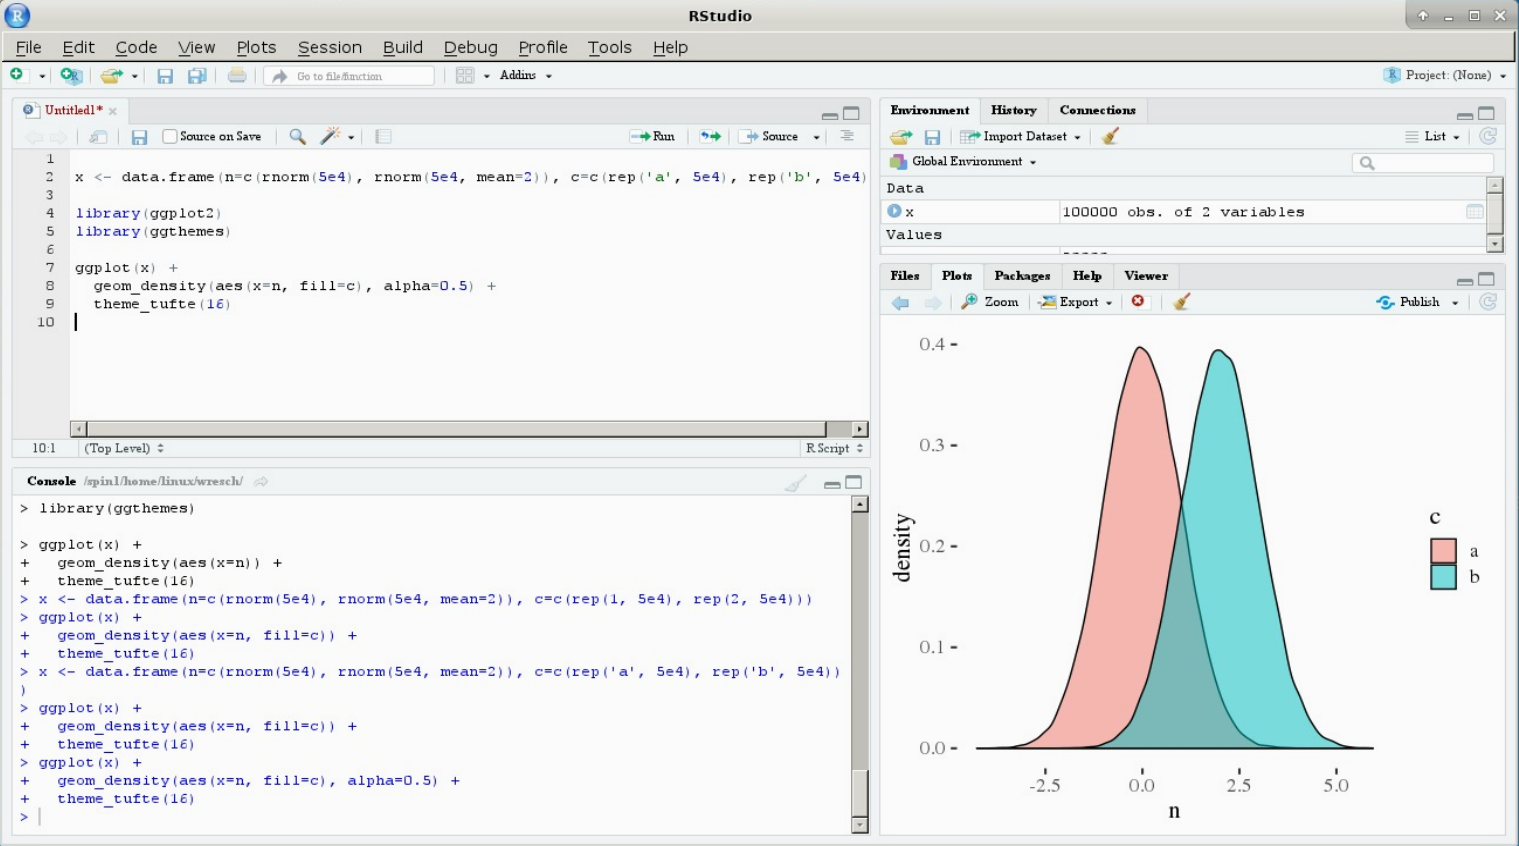
\includegraphics[scale=0.28]{rstudio_ide.png}
    \\[4cm]

    \begin{minipage}{0.4\textwidth}
      \begin{center} \large
        Lilian \textsc{RUSSO}\\
        Promo 2019/2020\\
      \end{center}
    \end{minipage}

  \end{center}
  \end{sffamily}
\end{titlepage}

\newpage

\begin{center}
    \textsc{\huge Introduction au document}\\[2cm]
\end{center} 

\paragraph{Ce document est un mémo qui regroupe normalement l'essentiel des notions vu en R. Il s'adresse principalement au étudiant de S4 INF/MAT/MIN mais peut servir de base de connaissance à toute personne souhaitant apprendre le langage R}

\paragraph{Il est fortement conseillé d'utiliser ce document sous format numérique. En effet, toutes les fonctions décrites dans le documents ont des liens vers des ressources officielles ont été mise pour plus d'approfondissement (le plus souvent sur le site du langage R), il vous suffut juste de cliquer dessus. Par exemple, vous pouvez cliquer sur mon adresse mail, cela ouvrira votre service de messagerie par défaut}

\paragraph{Par ailleurs, ce document étant fait par un seul étudiant non compétant dans sa propre langue maternelle, il se peut fortement que des fautes d'orthographes soit présentes. L'auteur se dédouane donc de toute hémorragie des yeux qui surviendrait lord de la lecture. Dans cette même continuité, il se peut que des ressources en lignes soit plus cohérentes où même que certaines présentes dans le documents soit obsolète.}

\paragraph{Pour toutes recommandation vissant a améliorer la qualité de ce document, je vous prie de me joindre sur mon mail : \href{mailto:lilianrussosup@gmail.com}{lilianrussosup@gmail.com}}

\newpage

\hspace{3cm}

\tableofcontents

\newpage
\section{Vecteur et matrice}
\subsection{Création et manipulation}
\subsubsection{Création}
On peut créer un vecteur de donnée à partir de la commande  :
\begin{minted}{R}
c(valeur1,valeur2,...)
\end{minted}
On peut créer une matrice avec les vecteurs de donnée x et y comportant z colonnes avec : 
\begin{minted}{R}
matrix(c(x,y),ncol=z)
\end{minted}

\subsubsection{Manipulation}
Affectation : 
\begin{minted}{R}
c(valeur1,...)->x
x=c(valeur1,...)
x<-c(valeur1,...)
\end{minted}
Extraire une donnée : 
\begin{minted}{R}
x[y] # pour obtenir l'élément d’indice y du vecteur x 
x[c(y,z)] # pour obtenir les éléments d’indices y et z.
x[-y]#retourne tout les éléments de x sauf celui à l'indice y
\end{minted}

\subsection{Manipulation sur un seul vecteur}
\subsubsection{Opération sur le vecteur par un scalaire}
Soit x = c(1,2,3,4,5)
\begin{minted}{R}
x/5 #(1/5,2/5,3/5,4/5,1)
x*5 #(5,10,15,20,25)
x+1 #(2,3,4,5,6)
x-1 #(0,1,2,3,4)
\end{minted}
\subsubsection{Somme}
\begin{minted}{R}
sum(x) #15
\end{minted}
\subsubsection{Somme cumulée croissant}
\begin{minted}{R}
cumsum(x) #1,3,6,10,15
\end{minted}

\subsubsection{Dimention du vecteur}
\begin{minted}{R}
length(x) #5
\end{minted}

\subsubsection{Racine}
\begin{minted}{R}
sqrt(x)
\end{minted}

\subsubsection{Calcul d'une puissance}
\begin{minted}{R}
x^2 #(1,4,9,16,25)
\end{minted}

\subsubsection{Agrandir un vecteur de données}
\begin{minted}{R}
c(x,6) #1 2 3 4 5 6
c(x,1,1,1,1,1) # 1 2 3 4 5 1 1 1 1 1
\end{minted}

\subsubsection{Séquences de nombres}
Si on veut une séquence de x a y avec un pas de z :
\begin{minted}{R}
seq(x,y,z)

seq(1,10,2) #1 3 5 7 9
seq(from=1,to=2,by=.2) #1.0 1.2 1.4 1.6 1.8 2.0
\end{minted}

\subsubsection{Test sur le vecteur de donnée}
Si on veut que le vecteur x respecte une condition logique :
\begin{minted}{R}
x(opérateur logique)

x>0 #TRUE TRUE TRUE TRUE TRUE

\end{minted}
Si on veut le nombre de composante de x qui vérifie l'opérateur logique alors on fait : 
\begin{minted}{R}
which(x(opérateur logique))

which(x>0) #1 2 3 4 5
\end{minted}

\subsection{Manipulation avec plusieurs vecteurs}
\subsubsection{Opération sur des vecteurs}
Si on veut faire une opération sur les $x_{i}$ valeurs avec les $y_{i}$ valeurs des vecteurs x et y (de même longueur)
\begin{minted}{R}
x+y
x-y
x*y
x/y
\end{minted}
\subsubsection{Réunir deux vecteurs}
\begin{minted}{R}
cbind(x,y) #Retourne la matrice avec dans la première colonne les valeurs de x 
#et dans la deuxième colonne les valeurs de y
rbind(x,y) #Retourne la matrice avec dans la première ligne les valeurs de x 
#et dans la deuxième ligne les valeurs de y
t(cbind(x,y)) #Transforme les lignes en colonne
t(rbind(x,y)) #Transforme les colonnes en lignes
\end{minted}

\subsection{Calcul sur les matrices}
\subsubsection{Somme}
\begin{minted}{R}
sum(A)#Somme toutes les valeurs de A
A+1 #+1 a toutes les valeurs de A
\end{minted}

\subsubsection{Produit}
\begin{minted}{R}
A*A #Chaque valeurs de A est multipliée par elle même
\end{minted}


\subsubsection{Produit matriciel}
\begin{minted}{R}
c(1,2)->a
A%*%a
t(a)%*%t(A) \#la colonne se transforme en ligne
\end{minted}
\newpage
\section{Graphique}

\subsection{Graphes de fonctions}\label{rappel bas/haut niveau}
Rappel : En LateX, il y a deux types de fonctions graphiques :
\begin{itemize}
    \item Celle de \textbf{bas niveau} qui font apparaître le tracé de la courbe en créant un nouvel environnement graphique.
    \item Celle de \textbf{haut niveau} qui ne font qu'ajouter le tracé de la fonction mais ne font pas de nouvel environnement graphique. 
\end{itemize}
\textbf{Il faut donc obligatoirement utiliser une fonction de bas niveau avant d'utiliser une fonction de haut niveau}
\subsubsection{Tracer les graphes de fonction : \href{https://www.rdocumentation.org/packages/graphics/versions/3.6.2/topics/plot}{plot()}}
Plot est une fonction de bas niveau permettant de tracer le graphe d'une fonction sur un intervalle donné (par défaut c'est celui des abscisse et ordonnées passée en paramètre) avec les arguments \argument{xlim} et \argument{ylim}
\begin{minted}{R}
plot(absice,ord,sub = "Nom du graphe",xlab = "Titre de l'axe des abscisse"
,ylab = "Titre de l'axe des ordonnées")
\end{minted}
\subsubsection{Tracer les graphes de fonction : \href{https://www.rdocumentation.org/packages/graphics/versions/3.6.2/topics/curve}{curve()} }
curve est une alternative à plot, la principale différence est qu'elle prend en premier paramètre le nom de la fonction voulue (définie par R) et permet de ne pas créer deux vecteurs abscisse et ordonnée au préalable. Elle est par contre plus compliquée a utiliser dans le cadre de fonction faites par l'utilisateur. A part les 3 premiers arguments qui changes (\argument{la fonction},\argument{Le point de départ},\argument{Le point de fin}) et le nom du graphique : \argument{xname}, le reste ne change pas par rapport à plot()
\begin{minted}{R}
curve(sin,0,7,xname = "Titre du graphe",xlab = "Titre de l'axe des absences",
ylab = "Titre de l'axe des ordonnés")
\end{minted}

\paragraph{On peut d'ailleur tracer plusieurs courbes avec la fonction curve sur le même graphique. Il suffit d'ajouter l'argument \argument{add=T} dans les fonctions curve a ajouter dans le même graphique.}

\subsubsection{Tracer des droites : \href{https://www.rdocumentation.org/packages/graphics/versions/3.6.2/topics/abline}{abline()} }
abline(a,b,h=NULL,v=NULL) est une fonction de haut niveau qui permet de tracer une droite selon plusieurs paramètres : 
\begin{itemize}
    \item a : L'ordonner a l'origine pour la droite. 
    \item b : La pente de la droite (b=1 $\rightarrow$ la courbe sera de la forme y = x+1)
    \item h : Ajoute une ligne horizontale tout au long du graphique en partant du point d’ordonnée h.
    \item v : Ajoute une ligne verticale tout au long du graphique en partant du point d’abscisse x
\end{itemize}

\subsubsection{Placer un point : \href{https://www.rdocumentation.org/packages/reddPrec/versions/0.4.0/topics/points}{points()}}
points(x,y) est une fonction de haut niveau qui permet d'ajouter un point de coordonnée x et y dans le graphique

\begin{minted}{R}
abs = c(seq(0,7,0.1))
ord = sin(abs)
plot(abs,ord,sub = "Graphe sinus",xlab = "Absice",ylab = "Ordonee")
curve(sin,0,7,xname = "Graphe sinus",xlab = "Abscice",ylab = "Ordonnee")
abline(h=1,col = "red")
abline(0,1,col="green")
abline(-1,1,col="yellow")
abline(v=1,col="pink")
points(3,1)
\end{minted}
\newpage
\begin{figure}[!h]
    \centering
    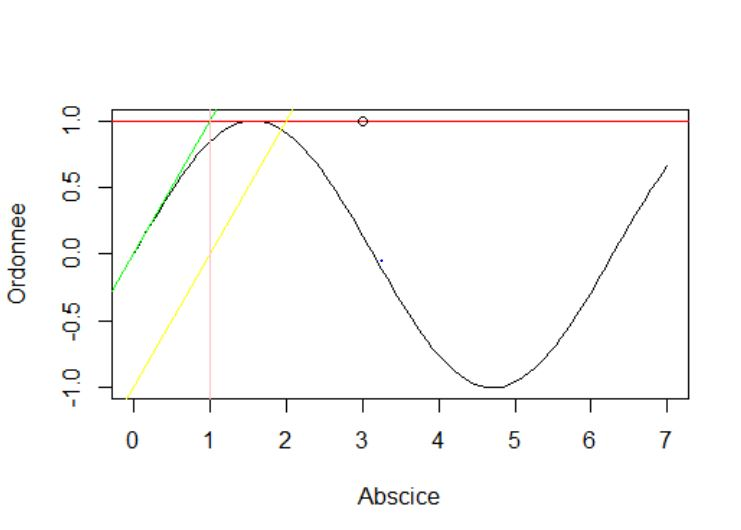
\includegraphics[scale=0.9]{exempleR.JPG}
\end{figure}
\paragraph{On peut voir ici une utilisation des 4 fonctions graphiques énoncées plus haut avec le résultat correspondant}
\subsubsection{Tracer des courbes de fonctions : \href{https://www.rdocumentation.org/packages/graphics/versions/3.6.2/topics/lines}{lines()}}\label{lines}
lines est une fonction de haut niveau permettant de tracer des courbes de fonctions, elle est généralement utilisée en complément de plot ou curve pour insérer une nouvelle fonction dans l'environnement

\begin{minted}{R}
absice = seq(-1.5,1.5,length.out = 1000)
ord = tan(absice)
plot(absice,ord,ylim = c(-1,7.5),xlim = c(-1.5,4.65),type = "l",xlab = "Absice",ylab = "Ordonee",sub = "Tangente")
absice2 = seq(1.65,4.65,length.out = 1000)
ord2 = tan(absice2)
lines(absice2,ord2,col="green")
\end{minted}


\begin{figure}[htbp]
    \centering
    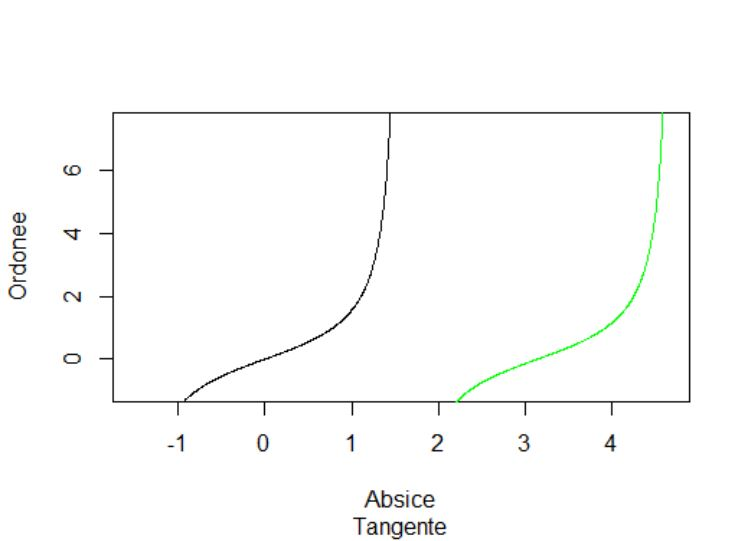
\includegraphics[scale=0.9]{graphe.JPG}
    \label{exemple_lines}
\end{figure}
\paragraph{On peut voir ici l'utilisation de lines() pour tracer la fonction de tangente sur un autre intervalle}
\newpage
\subsection{Graphes de données}
\subsubsection{Boite a moustache : \href{https://www.rdocumentation.org/packages/graphics/versions/3.6.2/topics/boxplot}{boxplot()} }
boxplot est une fonction qui convertis les données donnée en graphique appelé "boite à moustache". 
La boîte à moustaches résume seulement quelques indicateurs de position du caractère étudié (médiane, quartiles, minimum, maximum ou déciles). Ce diagramme est utilisé principalement pour comparer un même caractère dans deux populations de tailles différentes. \newline
On peut générer autant de boite a moustache que l'on veut sur le même graphique, il suffit juste des les mettres les uns a la suite des autres : boxplot(\argument{donnée 1},\argument{donnée 2},...)

\begin{minted}{R}
boxplot(mpg,main = "Boite à moustache",ylab="Consomation")
mtcars[am==0,"mpg"]->mpga
mtcars[am==1,"mpg"]->mpgm
boxplot(mpga,mpgm,names=c("automatique","manuelle"),main="mpg selon la transmission")
\end{minted}

\begin{figure}[!h]
    \centering
    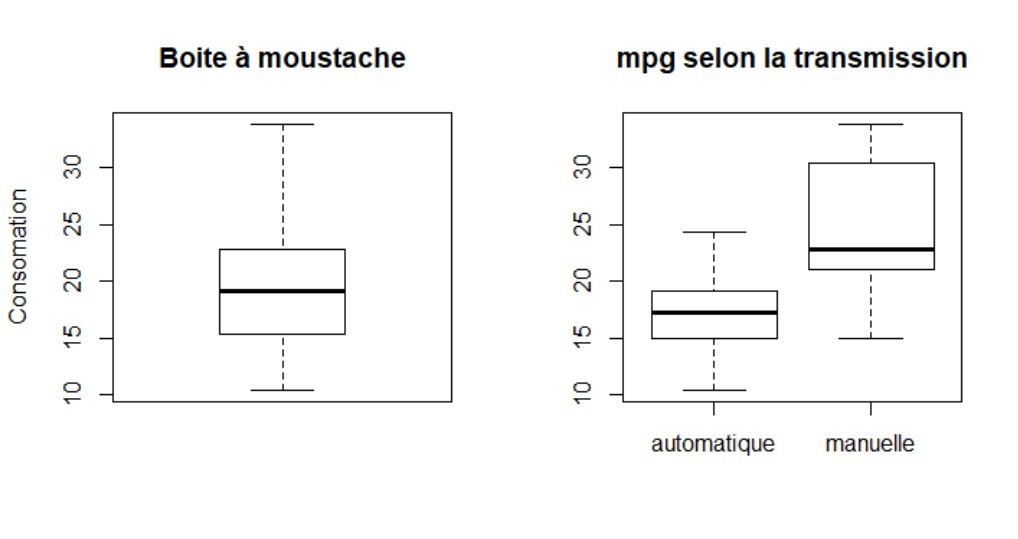
\includegraphics[scale=0.9]{image_moustache.JPG}
\end{figure}

\paragraph{On peut voir ici que les boites à moustaches peuvent êtres alignées, et le résultat de plusieurs jeu de donnée mise dans la même fonction}

\subsubsection{Graphique de secteur : \href{https://www.rdocumentation.org/packages/graphics/versions/3.6.2/topics/pie}{pie()} }
pie est la fonction pour tracer des graphiques à secteur (camembert) \newline
La fonction va convertir toutes les valeurs en pourcentage et réaliser le graphique associé. Les nom des valeurs de chaque partie de ce graphique correspond  Il est donc fortement recommander de l'utiliser avec des \textbf{variables quantitatives}

\begin{minted}{R}
pie(c(12,14,20))
\end{minted}

\begin{figure}[!h]
\centering
    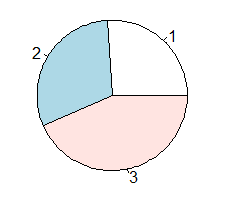
\includegraphics[scale = 0.6]{secteur.PNG}
\end{figure}

\newpage

\subsubsection{Diagramme en barre : \href{https://www.rdocumentation.org/packages/graphics/versions/3.6.2/topics/barplot}{barplot()} }
La fonction permet de tracer des diagrammes en barre en fonction d'un jeu de donnée fournie au préalable

\begin{minted}{R}
barplot(c(21,12,40))
\end{minted}

\begin{figure}[!h]
    \centering
    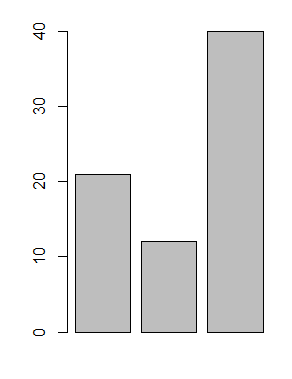
\includegraphics[scale = 0.5]{barre.PNG}
\end{figure}

\subsection{Option complémentaires}
\subsubsection{Colorer le graphe}\label{coloration}
Si on met plusieurs courbes dans un même graphique, il est souvent nécessaire de les différencier par la couleur. L'argument \argument{col} est à utiliser, comme dans l'exemple de la \textbf{fonction lines()}(\ref{lines}). Cependant, si on veut ajouter une légende ensuite, un autre choix s'avère plus judicieux : \textbf{remplacer les noms des couleurs par les chiffres correspondant.} Voici les correspondances des couleurs en R : 

\begin{figure}[!h]
    \centering
    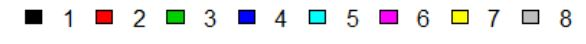
\includegraphics{palette.JPG}
    \label{fig:couleurs}
\end{figure}

\begin{minted}{R}
abline(h=1,col = "red")
abline(h=1,col = 2) #Équivalent

\end{minted}
R comporte beaucoup plus de couleurs que ces 8 là, mais ce sont les seules a avoir un chiffre correspondant. Un graphe avec plus de 8 courbes serait sans doute illisible, d'autant plus qu'il exite \href{http://www.sthda.com/french/wiki/les-differents-types-de-traits-dans-r-lty}{\textbf{d'autre moyens pour différencier deux courbes}}. \newline Pour le reste des couleurs prédéfinie (657 en tout), il faudra saisir leurs nom. Vous pourrez vous référer a la fonction colors() qui liste l'ensemble des couleurs définie dans R.
\begin{figure*}[!h]
    \centering
    
\includegraphics[scale = 0.18]{palette full.PNG}
    \label{fig:my_label}
    \caption*{Aperçu de l'ensemble des couleurs prédéfinies}
\end{figure*}

Mais ce n'est qu'une petite partie de l'ensemble des couleurs gérée par R. En effet, on peut spécifier le code hexadécimal d'une couleur : 
\mint{R}|barplot(c(2,5), col=c("#009999", "#0000FF"))|

\paragraph{Note : ce document ne traitera pas les autres package permettant de réaliser des palette de couleurs personnalisée. Si vous avez envie d'approfondir le sujet, je vous invite a vous rendre sur \href{http://www.sthda.com/french/wiki/couleurs-dans-r}{\underline{le site STHDA}} pour plus d'information}
\newpage


\subsubsection{Ajouter une légende : \href{http://www.sthda.com/french/wiki/ajouter-une-legende-aux-graphiques-avec-le-logiciel-r-comment-prendre-le-controle}{legend()}}

\warning{Attention : cette fonction fait partie du haut niveau (voir \ref{rappel bas/haut niveau}), elle nécessite donc un environnement déjà crée pour fonctionner. Par ailleurs, n'attendez rien d'automatique par cette fonction, elle se contente juste de récupérer les informations que vous lui fournissez et les places dans le graphique courrant}\newline Elle permet d'ajouter un petit encart à une position définie dans le graphique actuel. Il y a 4 principaux paramètre a définir : 
\begin{enumerate}
    \item \textbf{La position de la légende dans le graphique} : 
    \begin{figure}[!h]
        \centering
        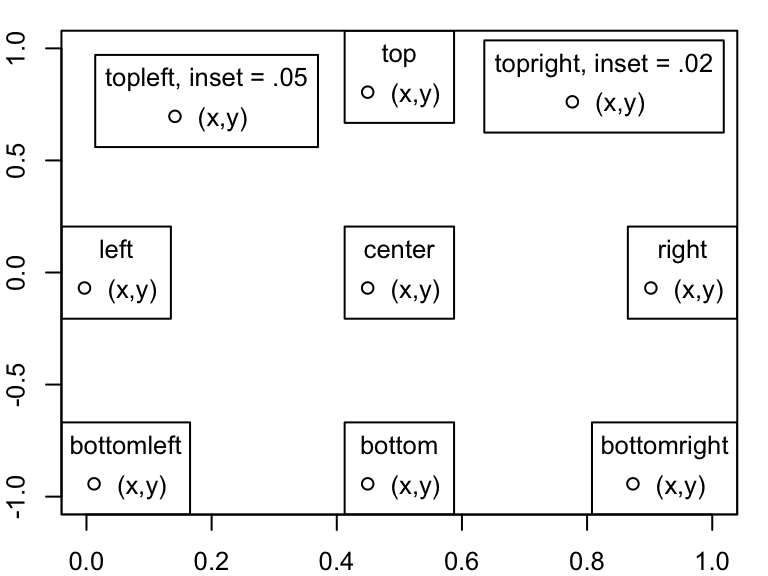
\includegraphics[scale=0.4]{add-legend-to-plot-legend-positions.png}
    \end{figure}
    \item \textbf{Les noms de chacune des légendes} :\newline On crée un vecteur avec les noms de chacune des courbes du graphique. \newline Par exemple, si on veut légender un graphique a deux courbe, on créera le vecteur suivant 
    \mint{R}|legends = c("<nom de la 1ere courbe>","<nom de la deuxième courbe>")|
    \item \textbf{Les couleurs correspondantes} : \newline On va saisir ici un vecteur de donnée correspondant au couleur des courbes du graphique. Si on a un graphique a 2 courbes, on saisira : 
    \mint{R}|col = c("<couleur de la 1ere courbe>","<couleur de la deuxième courbe>")|
    On peut évidement remplacer les noms par les codes hexadécimaux ou un entier si la couleur fait partie de la palette de base (voir \ref{coloration} pour plus d'information)
    \item \textbf{La forme des tracés correspondant} :\newline On va aussi indiquer la forme du tracé avec un vecteur d'entier représentant le paramètre \argument{lty} de chaque fonction.
    \begin{itemize}
        \item Si toutes les courbes on la même forme de tracé : \newline On saisit juste l'entier correspondant
        \mint{R}|lty=<entier>|
        \item Par contre, si il y a plusieurs valeurs pour lty, il faut soit les saisirs une par une, soit bien organiser son graphiques : \newline Si on saisit \mint{R}|lty = c(1,2)| alors la première courbe de la légende aura un lty = 1, la deuxiemme un lty = 2, la troisième un lty=1,... 
    \end{itemize}
    

\end{enumerate}
\newpage
\underline{Exemple récapitulatif : }\newline Si on veut une légende se trouvant en haut a gauche, avec 2 courbes se nommant tangente et arc-tengente, étant de couleurs réspéctives 3 et 4 (voir \ref{coloration}) et de lty 2 et 3 , on saisit : 
\begin{minted}{R}
legend("topleft",legend = c("tangente","arc-tengente"),col = c(3,4),lty=c(2,3))
\end{minted}
et on obtient : 

\begin{figure}[!h]
    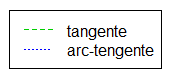
\includegraphics[scale=0.8]{legende.PNG}
\end{figure}

\paragraph{Il existe beaucoup d'autres paramètre pour la personification de la légende. Mais étant pour la plupart purement éstétique, ils ne seront pas traité dans ce document. Si vous voulez en savoir plus, \href{http://www.sthda.com/french/wiki/ajouter-une-legende-aux-graphiques-avec-le-logiciel-r-comment-prendre-le-controle}{\underline{le site STHSA}} est une très bonne ressource}

\subsection{Aligner plusieurs graphiques horizontalement ou verticalement : \href{https://www.datamentor.io/r-programming/subplot/}{par()}}
On dois parfois faire une comparaison de plusieurs graphiques, et les afficher sur le même environnement peut s'avérer utile. Pour cela, la fonction par(mfrow = c(\argument{x},\argument{y})) va diviser l'environnement. Le nouvel environnement aura \argument{x} lignes et \argument{y} colonnes. La disposition se fait automatiquement de gauche à droite et de haut en bas. \newline \textbf{Note : } Il existe beaucoup d'autres paramètres, dans un soucis de simplicité ils ne seront pas expliqué ici.\newline \underline{Exemple : }
\begin{minted}{R}
par(mfrow = c(2,1))
plot.new()
hist(c(3,4,1,2),main = "Graphe 1")
curve(sin,sub = "Graphe2")
\end{minted}
\begin{figure}[!h]
    \centering
    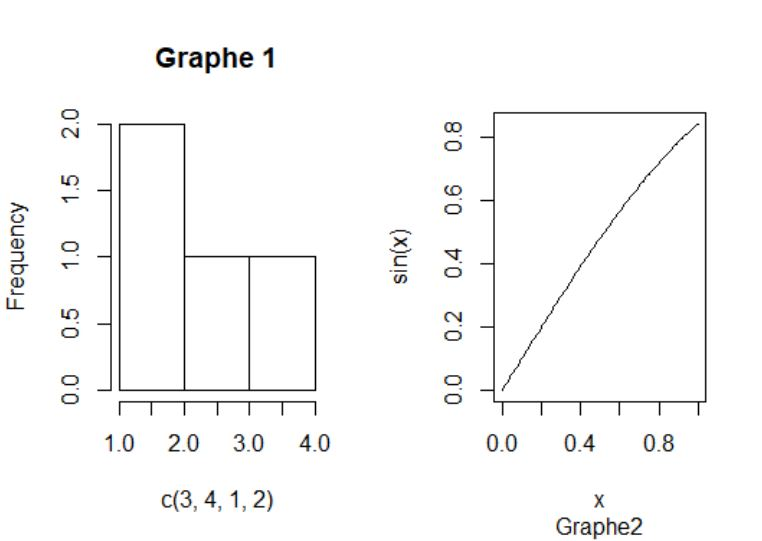
\includegraphics[scale = 0.7]{par.JPG}
\end{figure}

\newpage
\section{Statistiques descriptives}

\subsection{Premier aperçu des données}

\paragraph{Dans cette partie, j'utiliserai le package mtcars fournis de base par R. Ce dernier comporte diverses informations sur 32 voitures}

\subsubsection{Lister l'ensemble des données}

Pour afficher l'ensemble des données contenu dans la variable, il suffit juste de saisir le nom de la variable les contenant.
\begin{minted}{R}
mtcars # output : Tableau de 32 lignes et 11 colonnes
\end{minted}

\paragraph{Les données sont listées sous forme de colonnes, chacune représente une caractéristique}

\subsubsection{Récupérer le nom des colonnes : \href{https://www.rdocumentation.org/packages/base/versions/3.6.2/topics/name}{name()}}
La fonction retourne le nom de chaque colonnes du jeu de donnée. 
\begin{minted}{R}
name(mtcars) #output : "mpg" "cyl" "disp" "hp" "drat" "wt" "qsec" "vs" "am" "gear" "carb"
\end{minted}

\subsubsection{Avoir les 6 premières lignes de chaque colonnes : \href{https://www.rdocumentation.org/packages/utils/versions/3.6.2/topics/head}{head()} }
Pour avoir un apperçu de l'ensemble des données, on peut utiliser la fonction native head qui affiches les 6 premières lignes de chaque colonnes

\begin{minted}{R}
head(mtcars) #output : retourne un tableau de 6 lignes et 11 colonne
\end{minted}

\warning{Attention, ne pas confondre la fonction head avec la fonction summary, cette dernière renvois des informations sur les données}


\subsubsection{Premier résumé numérique : \href{https://www.rdocumentation.org/packages/base/versions/3.6.2/topics/summary}{summary()} }
On veut parfois avoir besoin d'indice sur chacune des colonne du jeu de donnée. La fonction summary a été créer pour ça : pour chaque colonne, elle revois : 
\begin{itemize}
    \item La plus petite valeur (Min.)
    \item Le premier quantile (1st Qu.)
    \item La médiane (Median)
    \item La moyenne (Mean)
    \item Le troisième quantile (3rd Qu.)
    \item La plus grande valeur (Max.)
\end{itemize}
Pour l'utiliser, il suffit de mettre en argument le jeu de donnée 
\begin{minted}{R}
summary(mtcars)
\end{minted}

\subsubsection{Extraire une variable d'un jeu de données}

\paragraph{Chaque colonnes d'un jeu de variables est une variable, représentant un vecteur de dimension n (le nombres de lignes totales du jeu de donnée.}Pour extraire une variable, on fait suivre le nom du jeu de donnée par le symbole \$ et du nom de la colonne à extraire. Par exemple si on veut extraire la colonne carb : 
\begin{minted}{R}
mtcars$carb #output : retourne les 32 valeurs de la colonne carb
\end{minted}

On peut ensuite utiliser ces valeurs pour créer des graphiques (voir $2^{eme}$ section)
\newpage

\subsubsection{Sélection conditionnelle, construction d'échantillon}
On peut sélectionner un ensembles de valeurs respectant des conditions données en arguments. \newline Par exemple, si on veut toutes les voiture qui sont automatiques (représenté par am == 0), on procède de la façon suivante : 
\begin{minted}{R}
mtcars[am==0,] #output : Renvois le nom de toutes les voitures ayant la valeurs 0 dans la colonne am
\end{minted}

\warning{Attention : ne pas oublier la "," après la condition}
\newline \newline
On peut évidement mettre plusieurs conditions dans la commande, il suffit de les mettre les unes a la suites des autres, séparé par un "\&".\newline Par exemple, pour avoir les véhicules non automatique (représenté par am == 1) et qui ont 8 cylindre (représenté par cyl == 8), on marque : 
\begin{minted}{R}
mtcars[cyl==8 & am==1,]
\end{minted}

On peut aussi ne sélectionner qu'une colonne parmit les résultats qu'on à obtenu.
\begin{minted}{R}
mtcars[am==0,"mpg"]
mtcars[am==0,]$mpg  #output : On a uniquement les valeurs de la colonnes mpg

\end{minted}
\paragraph{On peut utiliser cette méthode pour stocker le résultat dans une variables pour l'utiliser dans un graphe par exemple}

\subsection{Observation de la distribution des données}
\subsubsection{Sous forme d'effectif : \href{https://www.rdocumentation.org/packages/base/versions/3.6.2/topics/table}{table()} }
Cette fonction va retourner les effectifs de chaque valeurs d'un vecteur de données. C'est a utiliser pour \textbf{des variables qualitatives}.\newline Par exemple, pour obtenir le nombre de 0 et de 1 dans le vecteur de donnée am issue de mtcars : 
\begin{minted}{R}
table(am) #output : il y a 19 zero et 13 un
\end{minted}

\subsubsection{Sous forme de fréquences : \href{https://www.rdocumentation.org/packages/base/versions/3.6.2/topics/prop.table}{prop.table()}} 
La fonction va retourner les fréquences de chaque valeurs du vecteur de donnée dans un intervalle $[0;1]$\newline
\textbf{Cette fonction est très souvent utiliser avec la fonction table. En effet, elle récupère les données retourné par cette dernière et les transforme en fréquence}\newline Si on veut connaître les fréquences de 0 et de 1 dans le vecteur de donnée am issue de mtcars : 
\begin{minted}{R}
prop.table(table(am)) #output : il y a une proportion de 0.59375 zero et de 0.40625 un
\end{minted}
\argument{Note : } On peut redéfinir la fonction prop.table() : 
\begin{minted}{R}
table(am)/sum(table(am) #donne le même résultat
\end{minted}
\newpage

\section{Calcul de probabilité}
\subsection{Loi normale : $\mathcal{N}(\mu, {\sigma}^2)$}
Dans cette partie, on utilisera la loi normale \textbf{d'espérance} $\mu$ et \textbf{de variance ${\sigma}^2$} noté comme suit : $\mathcal{N}(\mu, {\sigma}^2)$\newline Il existe 4 fonctions principales : \newline \textbf{\large{\href{http://seankross.com/notes/dpqr/}{Pour cette partie, toutes les ressources sont centrée seankross}}}. C'est une ressource anglaise mais plutôt bien compréhensible.\newline
\underline{Note :} Si vous ne donner à la fonction que \argument{x}, alors par défaut \argument{y} = 0 et \argument{z} = 1 (loi normale centrée réduite)
\subsubsection{Calcul de la densité : pnorm()}

La fonction pnorm(\argument{x},\argument{y},\argument{z}) va nous donner la valeur $P(X \leq \argument{x})$ pour $X \sim \mathcal{N}(\argument{y}, {\argument{z}})$\newline Par exemple si on veut la probabilité pour que $X\leq 0$ avec $X \sim \mathcal{N}(0, 1)$ on peut marquer : \mint{R}|pnorm(0,0,1)| 
\vspace{0.3cm}
La fonction va vous aider à résoudre un problème de type : 
\begin{center}
    Calculer $P(X \in [\argument{a},\argument{b}])$ avec $\mu = \argument{x}$ et $\sigma = \argument{y}$
\end{center}
Pour ce faire : 
\begin{enumerate}
    \item on commence par définir nos deux variables mu et sigma : 
    \begin{minted}{R}
    mu = x
    sigma = y
    \end{minted}
    \item On calcule ensuite $P(X \leq \argument{b})$ : 
    \begin{minted}{R}
    pnorm(b,mean=mu,sd=sigma)
    \end{minted}
    \item On veut ensuite $P(X \geq \argument{a})$ : 
    \begin{minted}{R}
    pnorm((-a-mu)/sigma,x,y)
    \end{minted}
    \item Et enfin, on peut calculer $P(X \in [\argument{a},\argument{b}])$ avec $\mu = \argument{x}$ et $\sigma = \argument{y}$ : 
    \begin{minted}{R}
    pnorm(b,mu,sigma)-pnorm((-a-mu)/sigma,x,y)
    \end{minted}
\end{enumerate}
\subsubsection{Calculer les quantiles : qnorm()}
La fonction prend trois arguments : \argument{x}, \argument{y} et \argument{z}. Elle va calculer a pour $P(X \leq a) = \argument{x}$ avec $X \sim \mathcal{N}(\argument{y}, {\argument{z}})$.\newline Pour faire plus simple, la fonction va retourner le réel a partir du quel l'aire sous la courbe de la loi normale est égale à \argument{x}. Ce réel représente le point sur l'axe des abscisse ayant cette propriété
\newline \underline{Exemple :}\newline Si on veut la valeur a partir du quel l'aire sous la courbe est de 0.95 pour une loi normale $\mathcal{N}(3, 12)$(traduction mathématique : $P(X \leq a) = 0.95$, $X \sim \mathcal{N}(3, 12)$)
On peut écrire la fonction suivante : 
\mint{R}|qnorm(0.95,3,12)|
On trouve 22.73824. Donc $P(X \leq 22.73824) = 0.95$, $X \sim \mathcal{N}(3, 12)$)
\newline On peut d'ailleur calculer \textbf{plusieurs} quantile en même temps : 
\mint{R}|qnorm(seq(0.1,0.9,0.1),3,12)|
retourne tout les quantiles entre 0.1 et 0.9
\newpage
\subsubsection{Générateur aléatoire : rnorm()}
-rnorm(\argument{x},\argument{y},\argument{z}) va simplement retourner \argument{x} valeurs suivant la loi $\mathcal{N}(\argument{y}, \argument{z})$

\subsubsection{Calcul de la densité : dnorm()}
Si on veut calculer la densité d'un évènement avec une valeur donnée, on va utiliser dnorm(\argument{x},\argument{y},\argument{z}). On aura donc la densité au point \argument{x} de la loi $\mathcal{N}(\argument{y}, \argument{z})$
\end{document}